
\begin{figure*}[h]
%\subfigure[Figure A]{\label{fig:a}\includegraphics[width=60mm]{example-image-a}}
  \subfloat{
    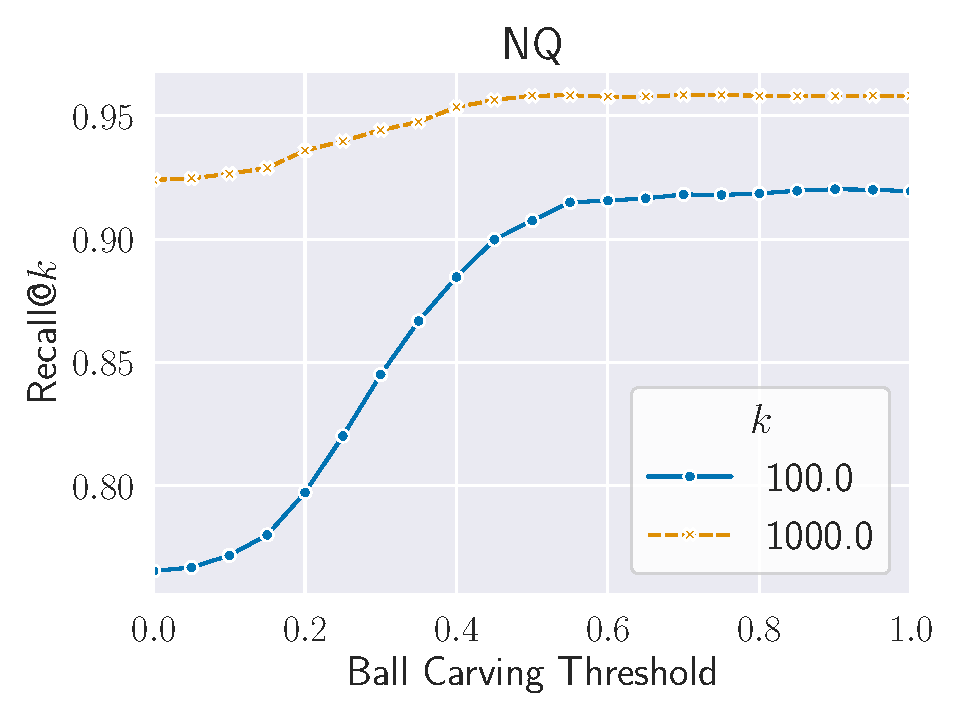
\includegraphics[width=.33\textwidth]{plots/NQ-ballcarvequality.pdf}}
  \subfloat{
    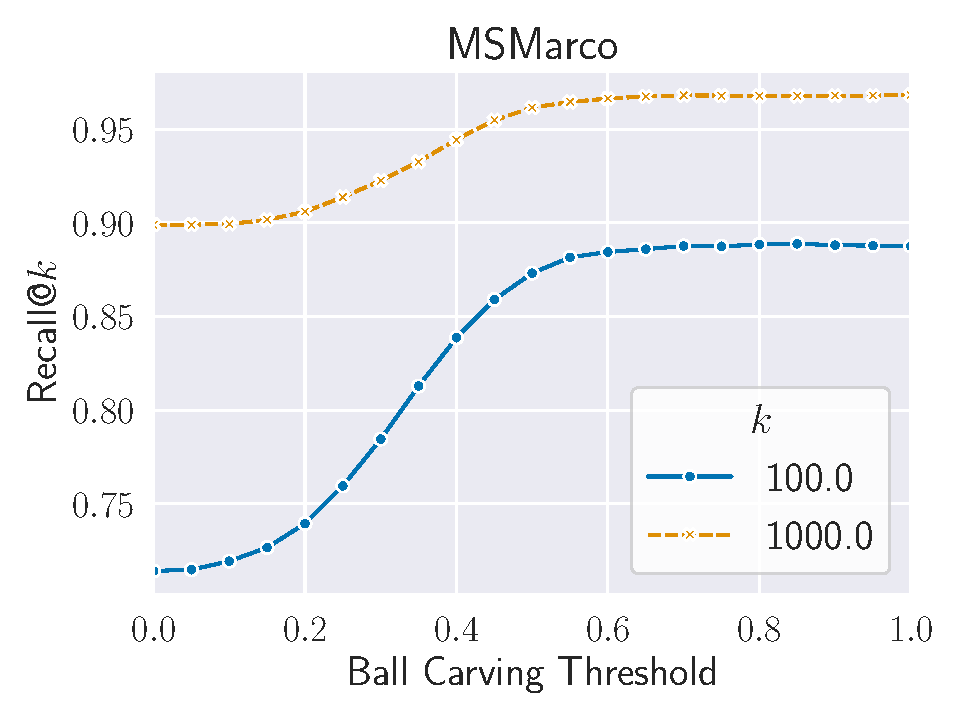
\includegraphics[width=.33\textwidth]{plots/MSMarco-ballcarvequality.pdf}}
  \subfloat{
    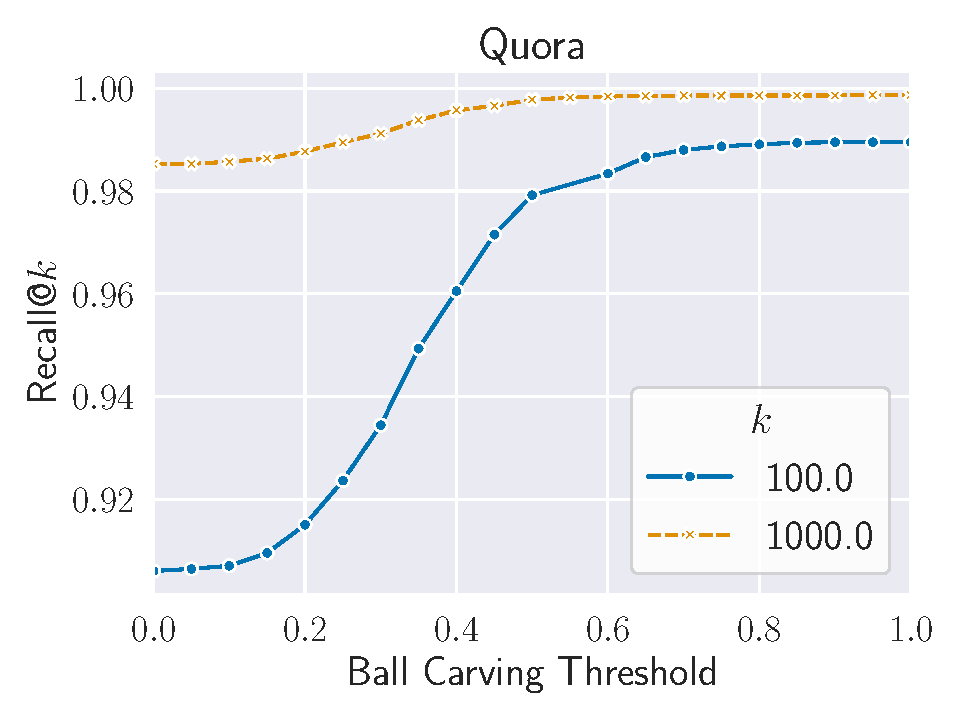
\includegraphics[width=.33\textwidth]{plots/Quora-ballcarvequality.pdf}}
\vspace{1em}
  \caption{\small Plots showing the trade-off between the threshold used for ball carving and the end-to-end recall.}
\label{fig:ballcarve}
\end{figure*}

\subsection{Ball Carving}\label{apx:ballcarve}
We now provide further details on the ball carving technique described in Section \ref{sec:online} that is used in our online experiments. Specifically, to improve rescoring latency, we reduce the number of query embeddings by a pre-clustering stage. Specifically, we group the queries $Q$ into clusters  $C_1,\dots,C_{k}$, set $c_i = \sum_{q\in C_i} q$ and $Q_C = \{c_1,\dots,c_{k}\}$. Then, after retrieving a set of candidate documents with the FDEs, instead of rescoring via $\CH(Q,P)$ for each candidate $P$, we rescore via $\CH(Q_C, P)$, which runs in time $O(|Q_C| \cdot |P|)$, offering speed-ups when the number of clusters is small. Instead of fixing $k$, we perform a greedy ball-carving procedure to allow $k$ to adapt to $Q$. Specifically, given a threshold $\tau$, we select an arbitrary point $q \in Q$, cluster it with all other points $q' \in Q$ with $\langle q,q'\rangle \geq \tau$, remove the clustered points and repeat until all points are clustered. 


In Figure \ref{fig:ballcarve}, we show the the trade-off between end-to-end Recall$@k$ of $\name$ and the ball carving threshold used. Notice that for both $k=100$ and $k=1000$, the Recall curves flatten dramatically after a threshold of $\tau = 0.6$, and for all datasets they are essentially flat after $\tau \geq 0.7$.  Thus, for such thresholds we incur essentially no quality loss by the ball carving. For this reason, we choose the value of $\tau = 0.7$ in our end-to-end experiments.

 On the other hand, we show that ball-carving at this threshold of $0.7$ gives non-trivial efficiency gains. Specifically, in Figure \ref{fig:BallCarveQPS}, we plot the per-core queries-per-second of re-ranking (i.e. computing $\CH(Q_C, P)$) against varying ball carving thresholds for the MS MARCO dataset. For sequential re-ranking, ball carving at a $\tau = 0.7$ threshold provides a $25\%$ QPS improvement, and when re-ranking is being done in parallel (over all cores simultaneously) it yields a 20$\%$ QPS improvement. Moreover, with a threshold of $\tau = 0.7$, there were an average of $5.9$ clusters created per query on MS Marco. This reduces the number of embeddings per query by 5.4$\times$, down from the initial fixed setting of $|Q| = 32$.  This suggests that pre-clustering the queries before re-ranking gives non-trivial runtime improvements with negligible quality loss.  This also suggests that a fixed setting of $|Q| = 32$ query embeddings per model is likely excessive for MV similarity quality, and that fewer queries could achieve a similar performance. 




\begin{figure}
    \centering
    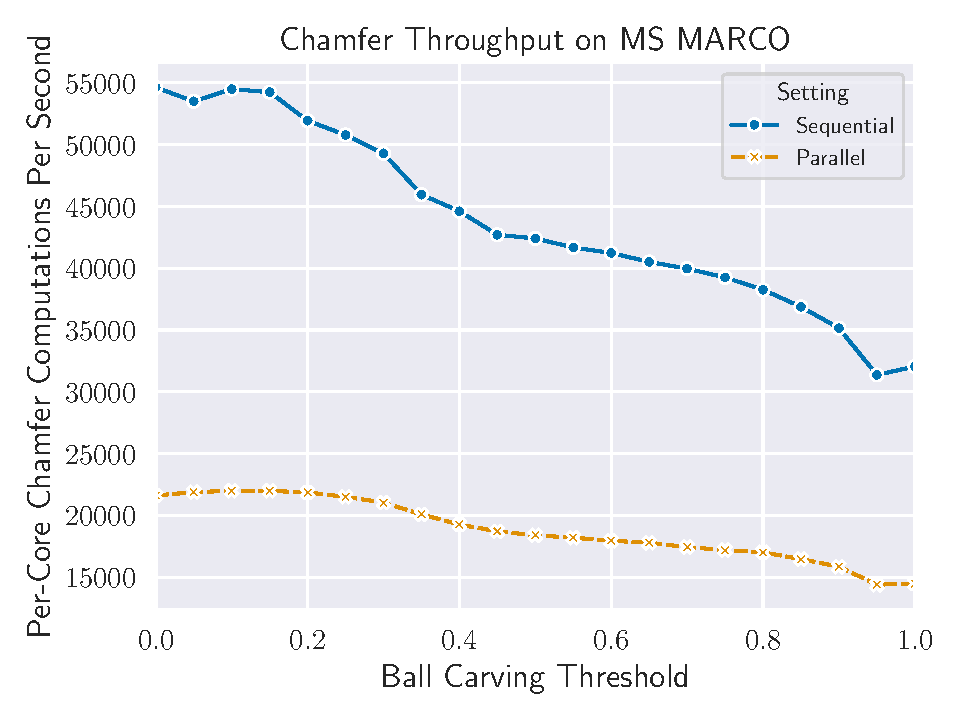
\includegraphics[scale = 0.4]{plots/BallCarvingQPS.pdf}
    \caption{Per-Core Re-ranking QPS versus Ball Carving Threshold, on MS MARCO dataset.}
    \label{fig:BallCarveQPS}
\end{figure}


\begin{figure*}[h]
  \subfloat{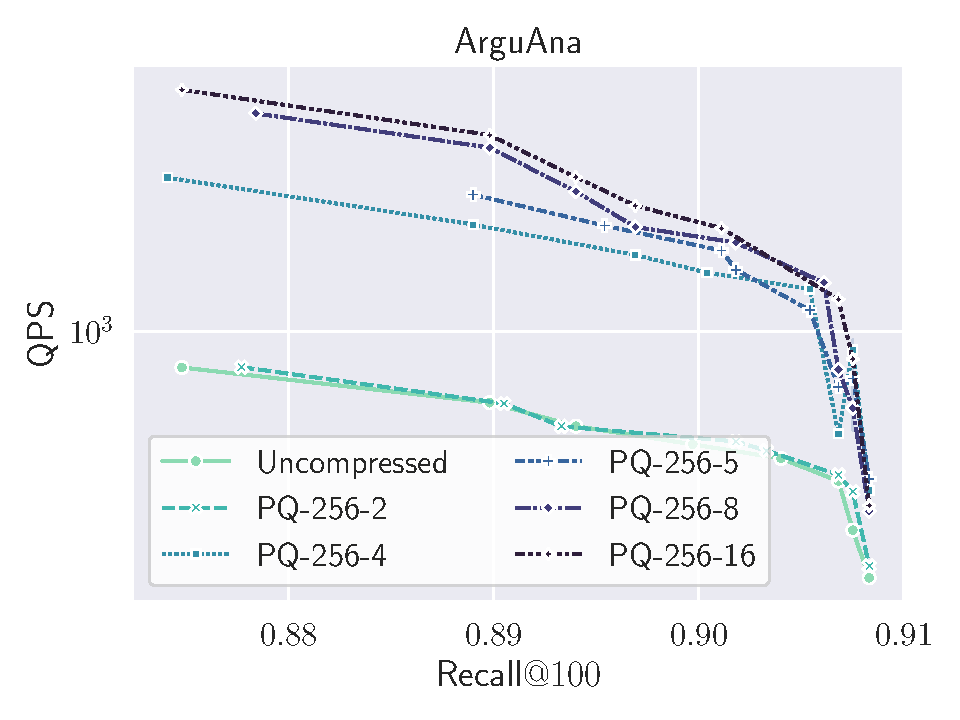
\includegraphics[width=.33\textwidth]{plots/pq_vs_qps_100/arguana-pq_vs_nopq.pdf}}
  \subfloat{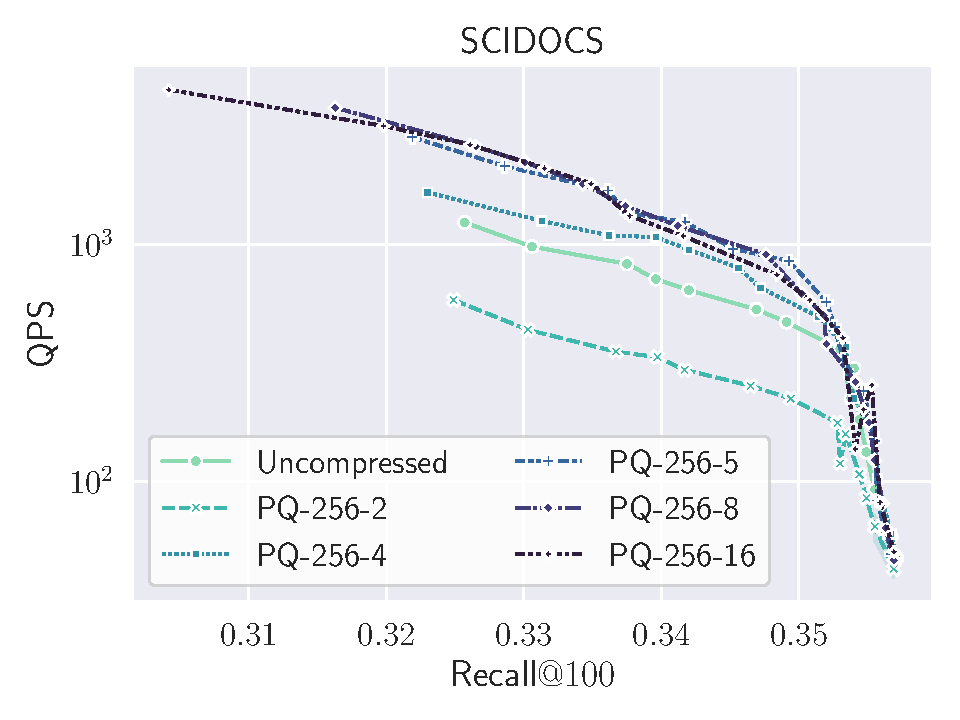
\includegraphics[width=.33\textwidth]{plots/pq_vs_qps_100/scidocs-pq_vs_nopq.pdf}}
  \subfloat{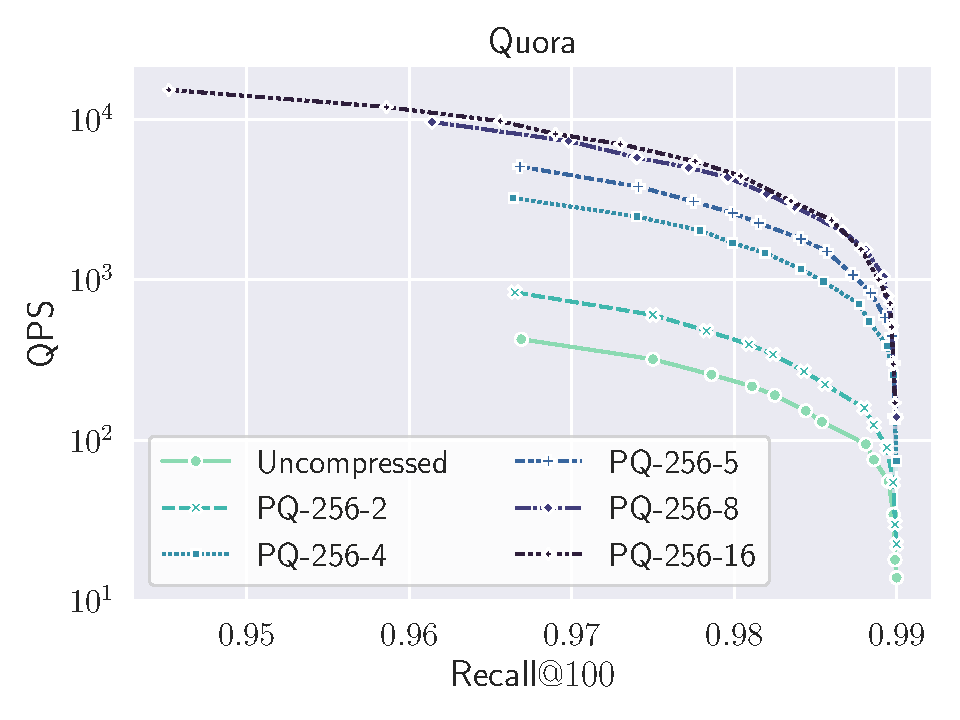
\includegraphics[width=.33\textwidth]{plots/pq_vs_qps_100/quora-pq_vs_nopq.pdf}}
  
  \subfloat{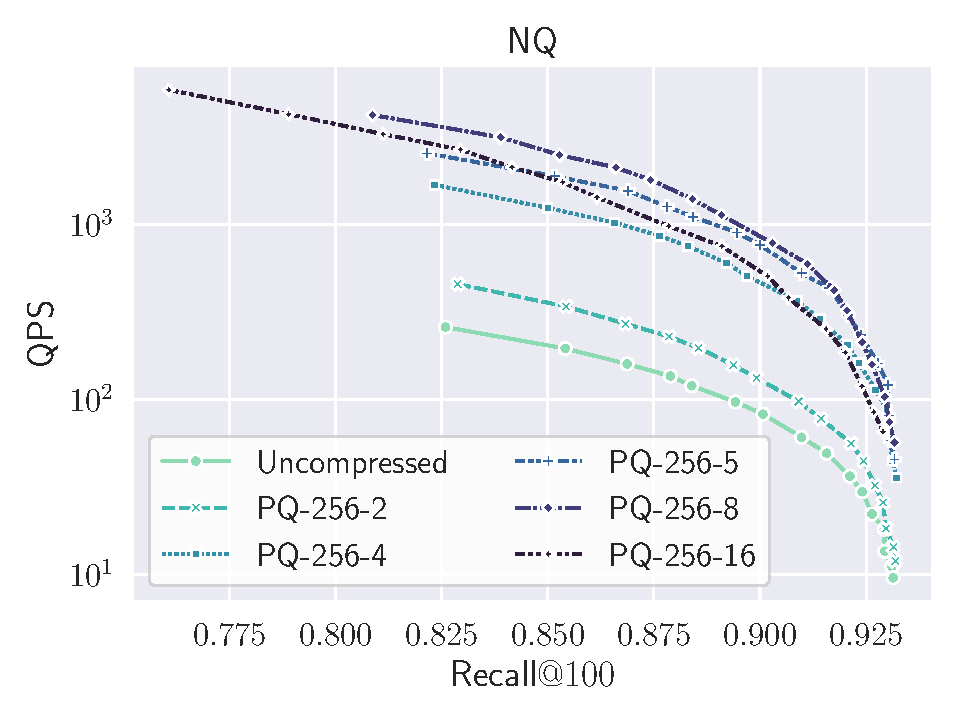
\includegraphics[width=.33\textwidth]{plots/pq_vs_qps_100/nq-pq_vs_nopq.pdf}}
  \subfloat{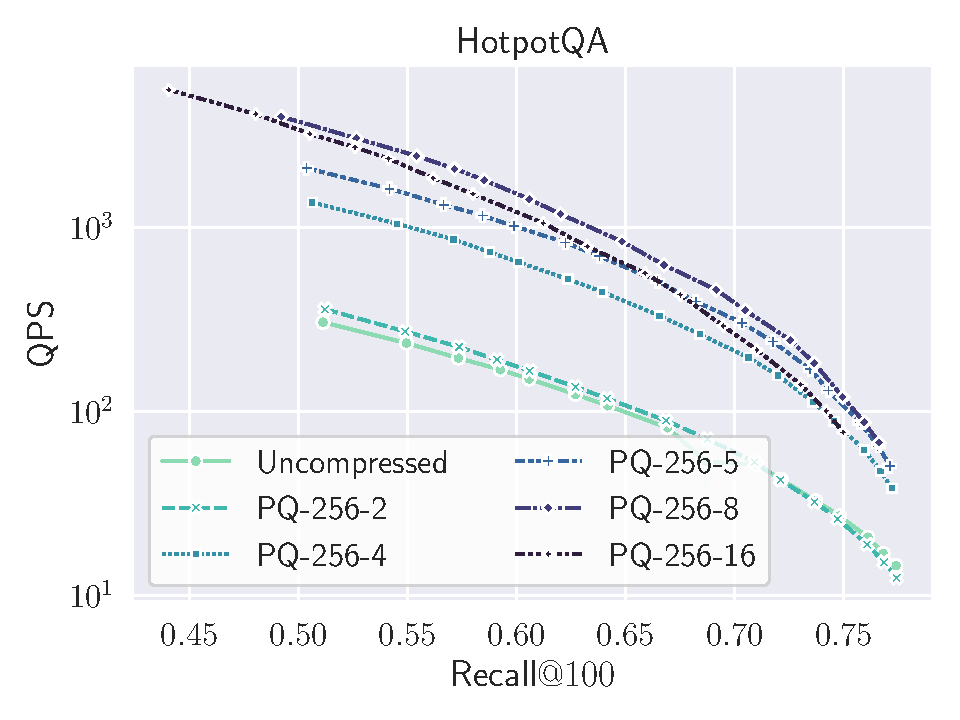
\includegraphics[width=.33\textwidth]{plots/pq_vs_qps_100/hotpotqa-pq_vs_nopq.pdf}}
  \subfloat{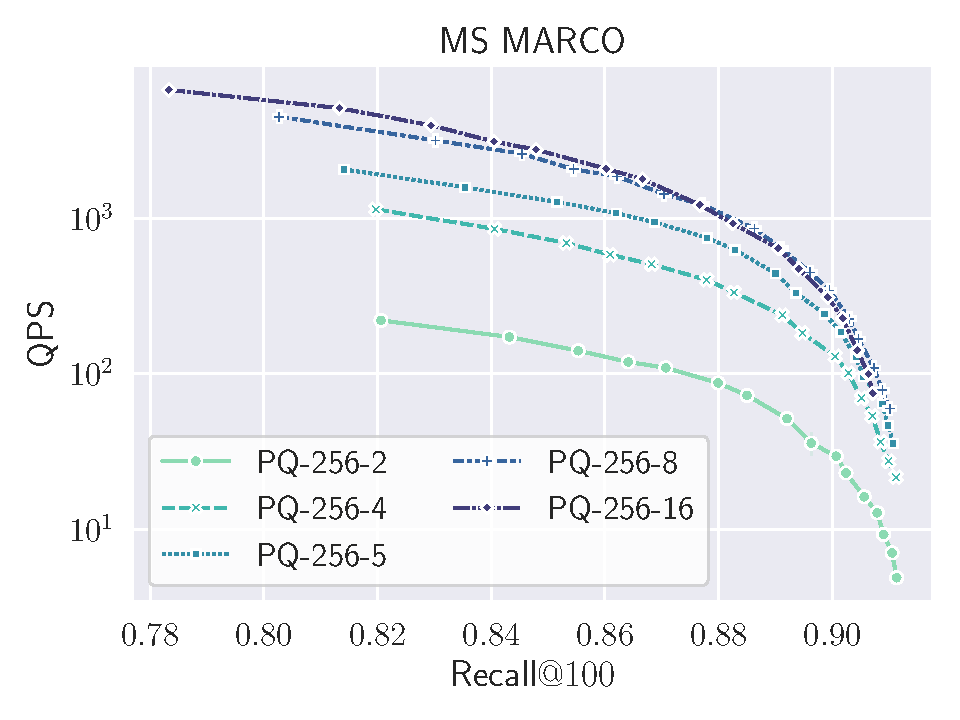
\includegraphics[width=.33\textwidth]{plots/pq_vs_qps_100/msmarco-pq_vs_nopq.pdf}}
  
\vspace{1em}
  \caption{\small Plots showing the QPS vs. Recall@$100$ for \name{} on the BEIR datasets we evaluate in this paper. The different curves are obtained by using different PQ methods on 10240-dimensional FDEs.}
\label{pq-qps-100-full}
\end{figure*}
\begin{figure*}[h]
  \subfloat{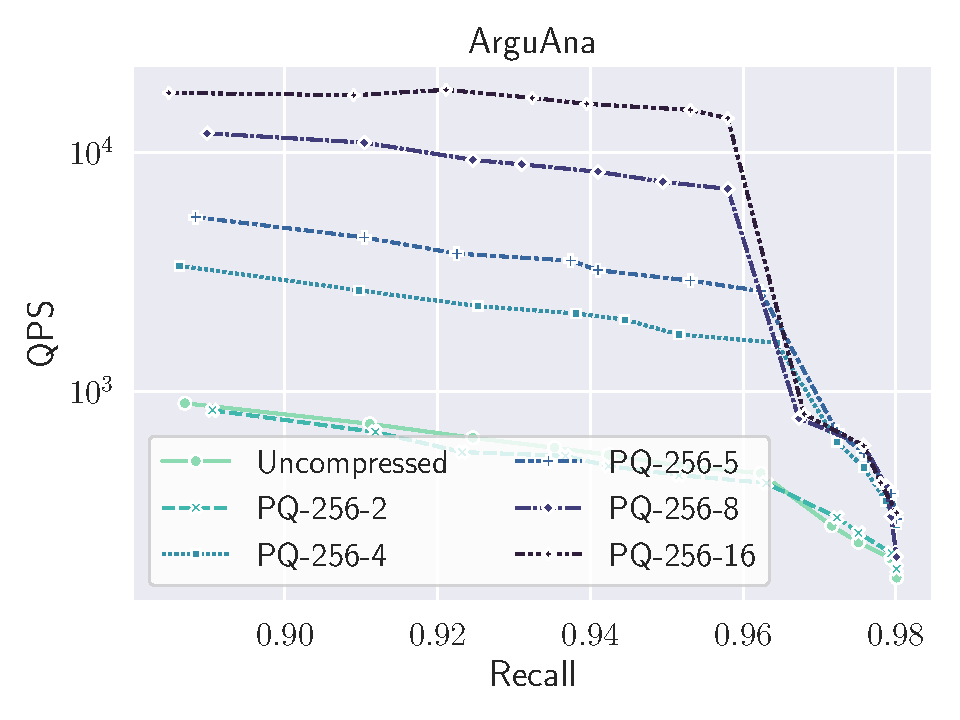
\includegraphics[width=.33\textwidth]{plots/pq_vs_qps_1k/arguana-1k-pq_vs_nopq.pdf}}
  \subfloat{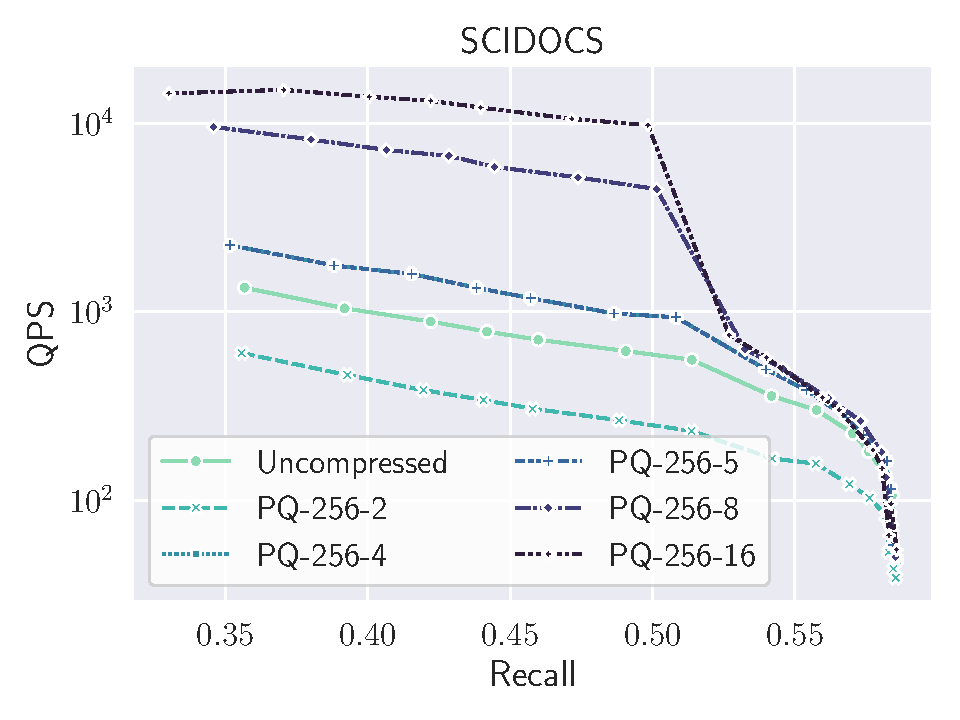
\includegraphics[width=.33\textwidth]{plots/pq_vs_qps_1k/scidocs-1k-pq_vs_nopq.pdf}}
  \subfloat{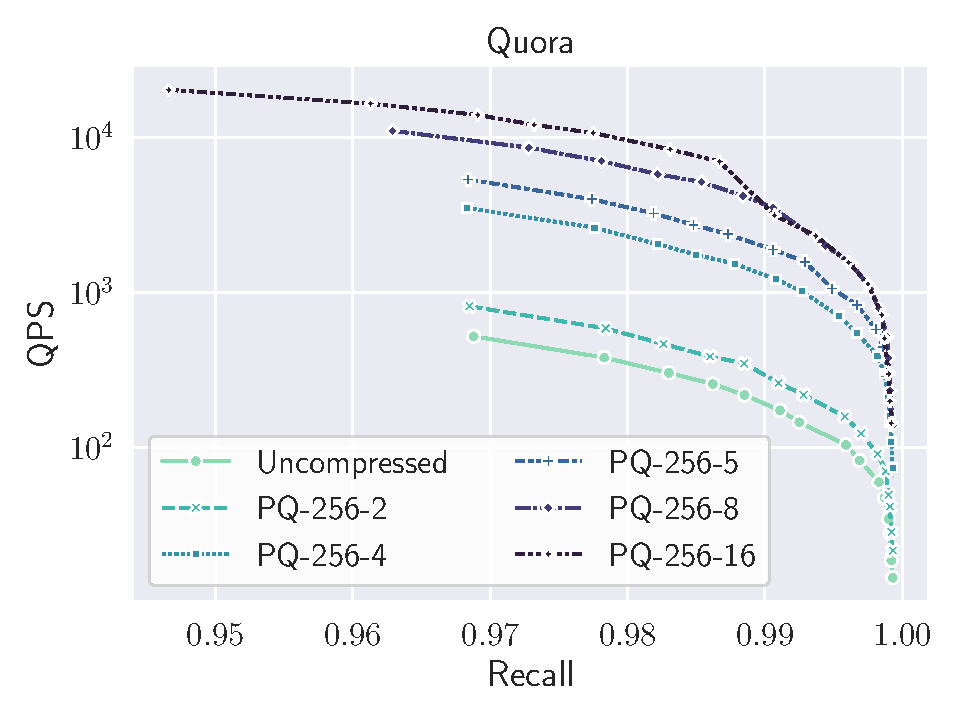
\includegraphics[width=.33\textwidth]{plots/pq_vs_qps_1k/quora-1k-pq_vs_nopq.pdf}}
  
  \subfloat{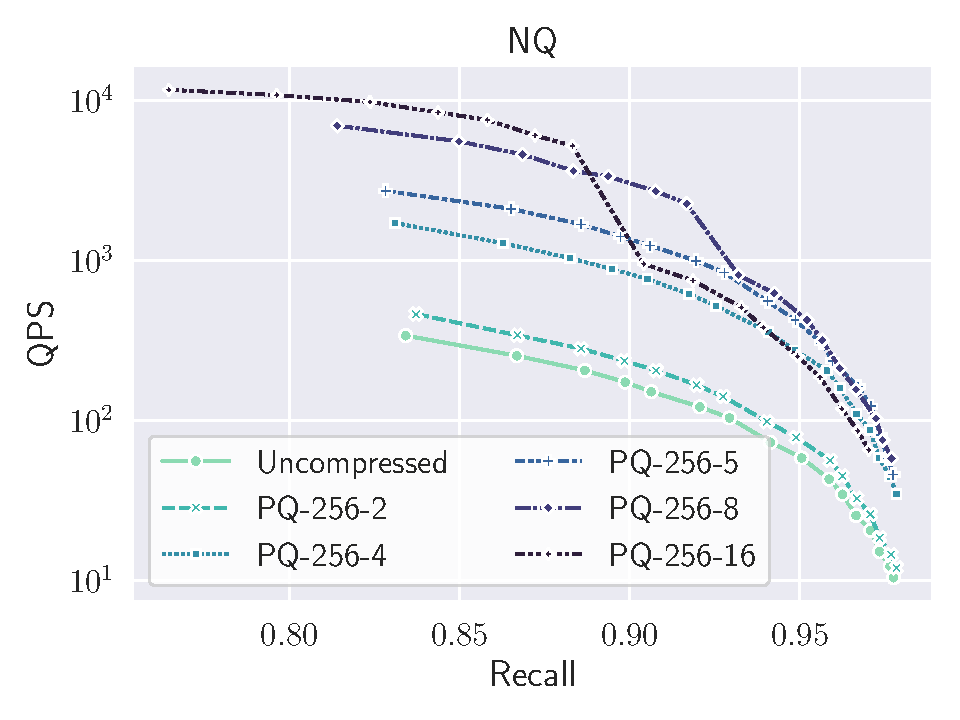
\includegraphics[width=.33\textwidth]{plots/pq_vs_qps_1k/nq-1k-pq_vs_nopq.pdf}}
  \subfloat{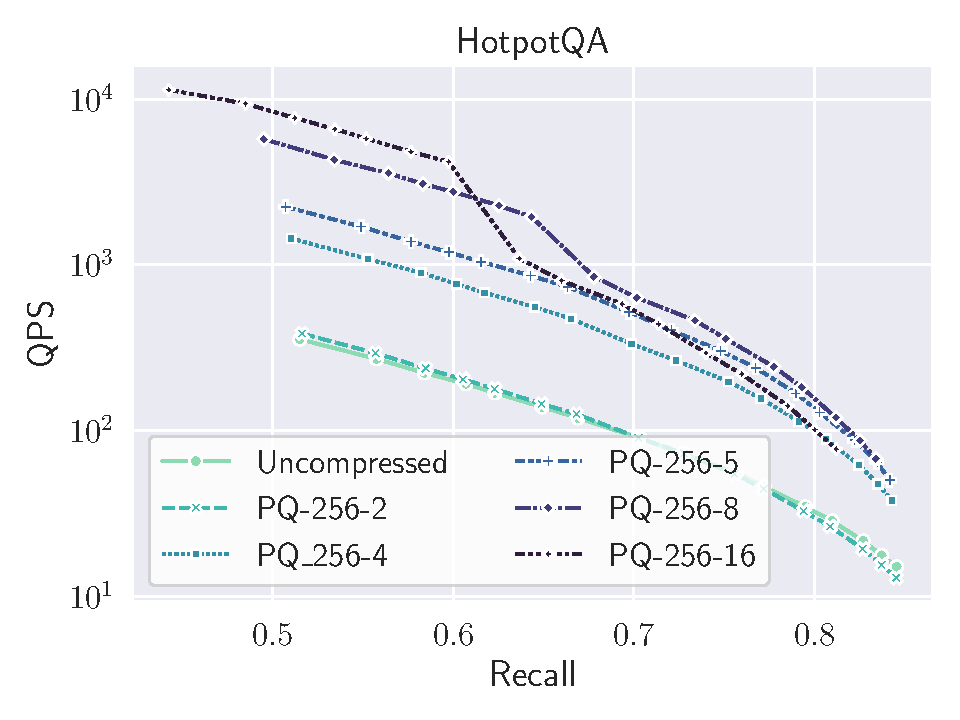
\includegraphics[width=.33\textwidth]{plots/pq_vs_qps_1k/hotpotqa-1k-pq_vs_nopq.pdf}}
  \subfloat{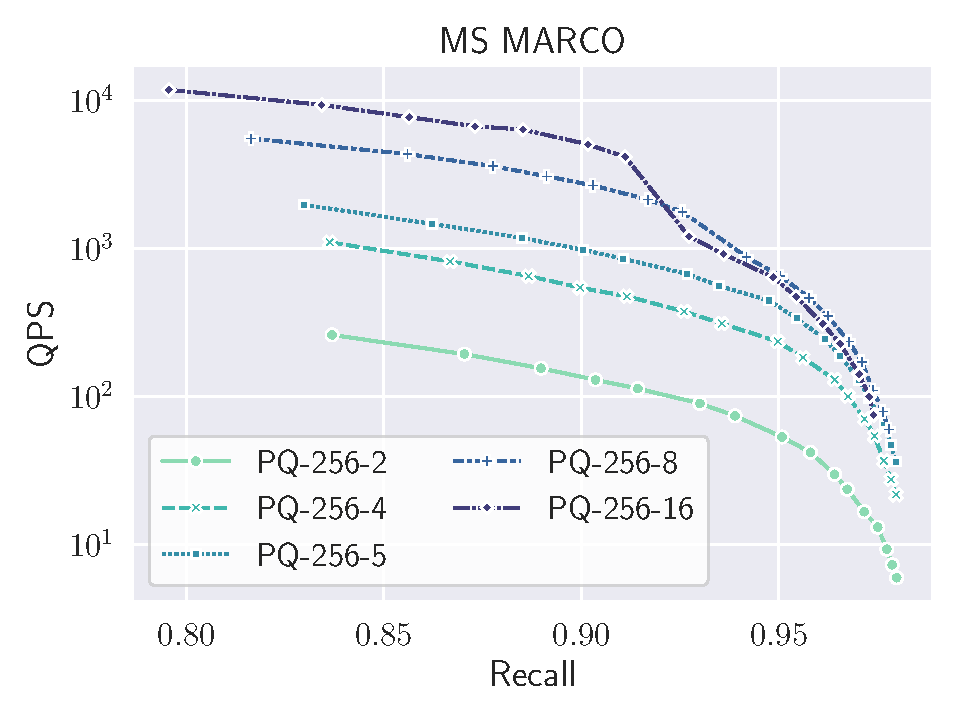
\includegraphics[width=.33\textwidth]{plots/pq_vs_qps_1k/msmarco-1k-pq_vs_nopq.pdf}} 
  
\vspace{1em}
  \caption{\small Plots showing the QPS vs. Recall@$1000$ for \name{} on the BEIR datasets we evaluate in this paper. The different curves are obtained by using different PQ methods on 10240-dimensional FDEs.}\label{pq-qps-1k-full}
\end{figure*}

\subsection{Product Quantization}\label{apx:PQ}
\paragraph{PQ Details} We implemented our product quantizers using a simple ``textbook'' $k$-means based quantizer. Recall that $\mathsf{AH}\text{-}C\text{-}G$ means that each consecutive group of $G$ dimensions is represented by $C$ centers. We train the quantizer by: (1) taking for each group of dimensions the coordinates of a sample of at most 100,000 vectors from the dataset, and (2) running $k$-means on this sample using $k=C=256$ centers until convergence. Given a vector $x \in \R^d$, we can split $x$ into $d/G$ blocks of coordinates $x_{(1)},\dots,x_{(d/G)} \in \R^G$ each of size $G$. The block $x_{(i)}$ can be compressed by representing $x_{(i)}$ by the index of the centroid from the $i$-th group that is nearest to $x_{(i)}$. Since there are $256$ centroids per group, each block $x_{(i)}$ can then be represented by a single byte.


\paragraph{Results} In Figures~\ref{pq-qps-100-full} and \ref{pq-qps-1k-full} we show the full set of results for our QPS experiments from Section~\ref{sec:online} on all of the BEIR datasets that we evaluated in this paper. We include results for both Recall@$100$ (Figure~\ref{pq-qps-100-full}) and Recall@$1000$ (Figure~\ref{pq-qps-1k-full}).

We find that $\mathsf{PQ}\text{-}256\text{-}8$ is consistently the best performing PQ codec across all of the datasets that we tested.
Not using PQ at all results in significantly worse results (worse by at least 5$\times$ compared to using PQ) at the same beam width for the beam; however, the recall loss due to using $\mathsf{PQ}\text{-}256\text{-}8$ is minimal, and usually only a fraction of a percent. 
Since our retrieval engine works by over-retrieving with respect to the FDEs and then reranking using Chamfer similarity, the loss due to approximating the FDEs using PQ can be handled by simply over-retrieving slightly more candidates.

We also observe that the difference between different PQ codecs is much more pronounced in the lower-recall regime when searching for the top $1000$ candidates for a query. For example, most of the plots in Figure~\ref{pq-qps-1k-full} show significant stratification in the QPS achieved in lower recall regimes, with  $\mathsf{PQ}\text{-}256\text{-}16$ (the most compressed and memory-efficient format) usually outperforming all others; however, for achieving higher recall, $\mathsf{PQ}\text{-}256\text{-}16$ actually does much worse than slightly less compressed formats like $\mathsf{PQ}\text{-}256\text{-}8$ and $\mathsf{PQ}\text{-}256\text{-}4$.


